%
% Modified by Megan Patnott
% Last Change: Jan 18, 2013
%
%%%%%%%%%%%%%%%%%%%%%%%%%%%%%%%%%%%%%%%%%%%%%%%%%%%%%%%%%%%%%%%%%%%%%%%%
%
% Modified by Sameer Vijay
% Last Change: Tue Jul 26 2005 13:00 CEST
%
%%%%%%%%%%%%%%%%%%%%%%%%%%%%%%%%%%%%%%%%%%%%%%%%%%%%%%%%%%%%%%%%%%%%%%%%
%
% Sample Notre Dame Thesis/Dissertation
% Using Donald Peterson's ndthesis classfile
%
% Written by Jeff Squyres and Don Peterson
%
% Provided by the Information Technology Committee of
%   the Graduate Student Union
%   http://www.gsu.nd.edu/
%
% Nothing in this document is serious except the format.  :-)
%
% If you have any suggestions, comments, questions, please send e-mail
% to: ndthesis@gsu.nd.edu
%
%%%%%%%%%%%%%%%%%%%%%%%%%%%%%%%%%%%%%%%%%%%%%%%%%%%%%%%%%%%%%%%%%%%%%%%%


%
% Chapter 1
%

\chapter{INTRODUCTION}
Airframe noise is significant

Landing gear is primary source of airframe noise

Health risks

\section{Motivation}
The present work is motivated to reduce noise by flow control via application of DBD plasma actuator technology.

\section{Theory of Aeroacoustics}
The modern theory of aeroacoustics, that is sound generated by aerodynamic means, is based on James Lighthill's so-called acoustic analogy. He states that sound generated in a fluid flow is only important in regions of turbulent fluctuations \cite{howe2003}. Based on this assumption, the Navier-Stokes Equation and isentropic equation of state are

\begin{equation} \label{eq:1-1}
	\frac{\partial \rho}{\partial t} + \frac{\partial(\rho u_i)}{\partial x_i} = 0
\end{equation}

	\begin{equation} \label{eq:1-2}
		\frac{\partial (\rho u_i)}{\partial t} + \frac{\partial(\rho u_i u_j + P_{ij})}{\partial x_j} = 0
	\end{equation}

\begin{equation}
	c_o^2 = \frac{\partial p}{\partial \rho}|_{s=const.} = \frac{p'}{\rho'}.
\end{equation}

\begin{equation}
\frac{\partial^2 \rho}{\partial t^2} - c_o^2 \nabla^2 \rho = \frac{\partial^2 T_{ij}}{\partial x_i \partial x_j}.
\end{equation}

\begin{equation}
T_{ij} = \rho u_i u_j + P_{ij} - c_o^2(\rho - \rho_0) \delta_{ij},
\end{equation}

where
\begin{equation}
\delta_{ij} = \left\{
\begin{array}{lcr}
1 & \mbox{if} & i = j \\
0 & \mbox{if} & i \neq j
\end{array}
\right\}
\end{equation}

\begin{equation}
T_{ij} \approxeq \rho_0 u_i u_j.
\end{equation}

\begin{equation}
p' = c_o^2 \rho' = \frac{1}{4\pi} \frac{\partial^2}{\partial x_i \partial x_j} \int_{V} \frac{T_{ij}}{r}dV,
\end{equation}

\begin{equation}
\int_{V} dV \propto D^3
\end{equation}

\begin{equation}
T_{ij} \propto \rho_o U_o^2
\end{equation}

\begin{equation}
\frac{\partial}{\partial x_i} = \frac{\partial}{c_o \partial t} \propto \frac{f}{c_o} \propto \frac{U_o}{c_o D}
\end{equation}

\begin{equation}
p' \propto \left( \frac{U_o}{c_o D} \right)^2 \left( D^3 \right) \left( \frac{\rho_o U_o^2}{r} \right) \propto \frac{U_o^4}{r}
\end{equation}

\begin{equation}
W \propto p'^2 \propto \frac{U_o^8}{r^2}
\end{equation}

\begin{equation}
p' = \underbrace{ \frac{1}{4\pi} \frac{\partial^2}{\partial x_i \partial x_j} \int_V \left[ \frac{T_{ij}}{r} \right] dV }_I - \underbrace{ \frac{1}{4\pi} \frac{\partial}{\partial x_j} \int_S \left[ \frac{P_{ij} + \rho v_i v_j}{r} \right] n_i dS }_{II} + \underbrace{ \frac{1}{4\pi} \frac{\partial}{\partial t} \int_S \left[ \frac{\rho v_i}{r} \right] n_i dS}_{III},
\end{equation}

\begin{equation}
II : \frac{1}{4\pi} \frac{\partial}{\partial x_j} \int_S \left[ \frac{P_{ij} + \rho v_i v_j}{r} \right] n_i dS \propto \left( \frac{U_o}{c_oD} \right) \left( \frac{\rho_o U_o^2}{r} \right) \left( D^2 \right) \propto \frac{U_o^3}{r}
\end{equation}

\begin{equation}
III : \frac{1}{4\pi} \frac{\partial}{\partial t} \int_S \left[ \frac{\rho v_i}{r} \right] n_i dS \propto \left( \frac{U_o}{D} \right) \left( \frac{\rho_o U_o}{r} \right) \left( D^2 \right) \propto \frac{U_o^2}{r}.
\end{equation}

\begin{equation}
II : W \propto p'^2 \propto \frac{U_o^6}{r^2},
\end{equation}

\begin{equation}
III : W \propto p'^2 \propto \frac{U_o^4}{r^2}.
\end{equation}

\section{Landing Gear}

\subsection{Geometry}

\subsection{Noise Sources}

\section{Literature Review}

\subsection{Single Cylinder Plasma Flow Control}

\subsection{Tandem Cylinders Plasma Flow Control}

\subsection{Shock Strut-Torque Arm Assembly Plasma Flow Control}

%Table~\ref{tbl:bogus1} shows some feeding frequencies for where Gnus
%like to eat around the Notre Dame campus.  Gnus have work weeks, just
%like humans do, hence the much lower frequencies on weekends.  This
%can lead us to conclude that Gnu weekend shifts are much smaller than
%the normal work-week shifts.  In fact, we can attempt to parametrize the
%sighting frequency, $\mathcal{F}$, by the student population, type of food, and
%day of the week as:
%\begin{equation}
%  \mathcal{F} = \mathcal{F}(p,f,d).
%\end{equation}
%Table~\ref{tbl:bogus2} shows what they
%typically like to eat.
%
%\begin{table}[tpb]
%  \begin{center}
%    \caption{WHERE Gnus LIKE TO EAT \label{tbl:bogus1}}
%    \begin{tabularx}{0.85\textwidth}{lrrrrrrr} \toprule
%      \multicolumn{1}{c}{Location} & Sun & Mon & Tue & Wed & Thu & Fri & Sat \\ \midrule
%      Front of Dome & 1 & 5 & 6 & 5 & 4 & 5 & 1 \\
%      Stonehenge & 2 & 9 & 10 & 12 & 9 & 14 & 2 \\
%      The Rock & 1 & 3 & 4 & 3 & 4 & 3 & 0 \\
%      The ACC & 3 & 4 & 5 & 5 & 5 & 4 & 1 \\
%      Dining Halls & 5 & 14 & 12 & 13 & 14 & 12 & 3 \\
%      Hesburgh Library & 2 & 3 & 5 & 2 & 3 & 4 & 2 \\ \bottomrule
%    \end{tabularx}
%  \end{center}
%\end{table}
%
%\begin{table}[tpb]
%  \setlength{\capwidth}{0.7\textwidth}
%  \begin{center}
%    \caption{WHAT Gnus LIKE TO EAT ON THE NOTRE DAME CAMPUS, LISTED
%      BY AVERAGE NUMBER OF SIGHTINGS PER WEEKDAY
%    \label{tbl:bogus2}
%}
%    \begin{tabular}{lrrrrrrr} \toprule
%      \multicolumn{1}{c}{Food} & Sun & Mon & Tue & Wed & Thu & Fri & Sat \\ \midrule
%      Twinkies & 1 & 5 & 6 & 5 & 4 & 5 & 1 \\
%      Ding Dongs & 2 & 9 & 10 & 12 & 9 & 14 & 2 \\
%      Carrots & 1 & 3 & 4 & 3 & 4 & 3 & 0 \\
%      Lettuce & 3 & 4 & 5 & 5 & 5 & 4 & 1 \\
%      Twizlers & 5 & 14 & 12 & 13 & 14 & 12 & 3 \\
%      Jawbreakers & 2 & 3 & 5 & 2 & 3 & 4 & 2 \\ \bottomrule
%    \end{tabular}
%  \end{center}
%\end{table}
%
%Figure~\ref{fig:bogus3} shows a nice graph of location distributions
%by day of week.  I have no real reason for including it except to show
%that figures work as well.  Did I mention that Gnus are really cool?
%
%\begin{figure}[tpb]
%  \begin{center}
%    \centerline{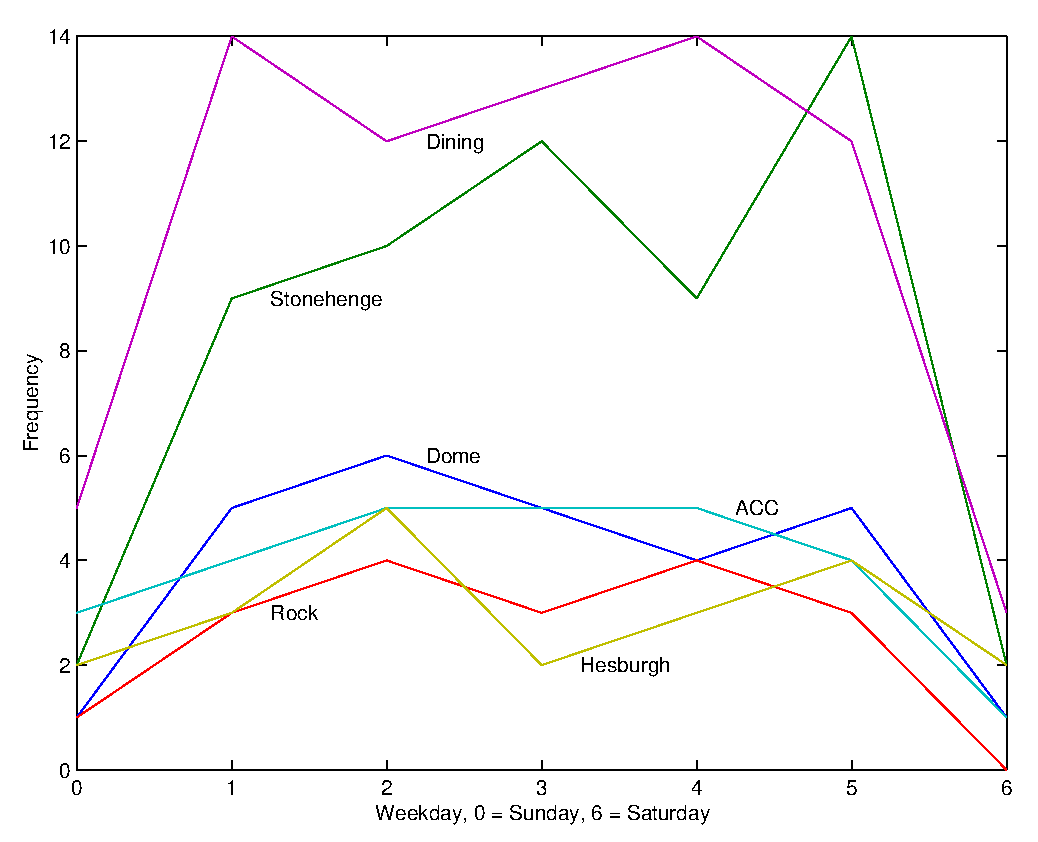
\includegraphics[scale=0.8]{sample_nd}}
%    \caption{Location distributions by day of where, where the X axis
%      is the weekday (0 through 6), and the Y axis is the sighting
%      frequency}
%    \label{fig:bogus3}
%  \end{center}
%\end{figure}
%
%Gnus typically tend to come out when there are large gatherings of
%humans with food.  Gnus work very hard at providing us with all the
%things that we like (trees, dirt, air, etc.), and so we should freely
%give them food.  They will come up and stand a respectful distance
%away from you, waiting to see if they will be rewarded for their
%efforts.  If you offer some food, they will take it and back off a
%respectful distance in order to consume their food while leaving you
%to your ``personal space.''

%\section{Groovin' Gnus}
%\label{sec:groovin-gnus}
%
%Gnus do tend to stay away from humans in their normal day-to-day
%workings.  This is mainly because humans don't, for the most part,
%understand what they are doing.  If a Gnu is working, and a human
%approaches it, the Gnu will tend to drop whatever it is doing and run
%away.  This is probably do to the tendency for humans to have ``group
%meetings'' and ``productivity seminars.''  Most Gnus are deathly
%afraid of such overmanagement, and run at the slightest hint of it,
%for fear that it will cripple their real work.
%
%It is interesting, however, that Gnus have chosen an Institution of
%Higher Education for their BOO.\footnote{Base of Operations.}  It is
%often said that:
%\begin{quote}
%  Academic politics are the dirtiest, meanest, ugliest, and generally
%  the most low-down, in-your-face, and kick-em-while-they're-down than
%  anywhere else (even Washington D.C.)  because the stakes are so low.
%\end{quote}
%It has been hypothesized that the Gnus are subtly trying to affect a
%change for the better (i.e., eliminating the overmanagement problems)
%by working the very system that they are trying to change, from
%within.  That is, the graduates from Notre Dame can learn from the
%examples of the Gnus here, and run screaming (or chattering) at the
%slightest hint of overmanagement, and let the real work proceed
%unhindered.

% % uncomment the following lines,
% if using chapter-wise bibliography
%
% \bibliographystyle{ndnatbib}
% \bibliography{example}
